% -*- compile-command: "rubber --unsafe -d disco-tfpie23.tex" -*-

\documentclass[submission,copyright,creativecommons]{eptcs}
\providecommand{\event}{TFPIE 2023} % Name of the event you are submitting to

%%%%%%%%%%%%%%%%%%%%%%%%%%%%%%%%%%%%%%%%%%%%%%%%%%%%%%%%%%%%
%% Package imports
%%%%%%%%%%%%%%%%%%%%%%%%%%%%%%%%%%%%%%%%%%%%%%%%%%%%%%%%%%%%

\usepackage{iftex}
\usepackage{underscore}         % Only needed if you use pdflatex.
\usepackage[T1]{fontenc}        % Recommended with pdflatex
\usepackage[utf8]{inputenc}
\usepackage{stmaryrd}
\usepackage{amsmath}
\usepackage{amssymb}
\usepackage{xspace}
\usepackage{prettyref}
\usepackage{xcolor}
\usepackage{minted}
\usepackage[all]{xy}
\usepackage{amsfonts}
\usepackage{graphicx}

%%%%%%%%%%%%%%%%%%%%%%%%%%%%%%%%%%%%%%%%%%%%%%%%%%%%%%%%%%%%
%% Semantic markup
%%%%%%%%%%%%%%%%%%%%%%%%%%%%%%%%%%%%%%%%%%%%%%%%%%%%%%%%%%%%

\newcommand{\disco}{\textsc{Disco}\xspace}

\newcommand{\term}[1]{\emph{#1}}

\newcommand{\pkg}[1]{\texttt{#1}}
\newcommand{\ext}[1]{\texttt{#1}}
\newcommand{\module}[1]{\texttt{#1}}

\newcommand{\ie}{\emph{i.e.}\ }
\newcommand{\eg}{\emph{e.g.}\ }
\newcommand{\etal}{\emph{et al.}\xspace}
\newcommand{\etc}{\emph{etc.}\xspace}

%%%%%%%%%%%%%%%%%%%%%%%%%%%%%%%%%%%%%%%%%%%%%%%%%%
% Prettyref
%%%%%%%%%%%%%%%%%%%%%%%%%%%%%%%%%%%%%%%%%%%%%%%%%%

\newrefformat{fig}{Fig.~\ref{#1}}
\newrefformat{sec}{Sect.~\ref{#1}}
\newrefformat{eq}{Equation~\eqref{#1}}
\newrefformat{prob}{Problem~\ref{#1}}
\newrefformat{tab}{Table~\ref{#1}}
\newrefformat{thm}{Theorem~\ref{#1}}
\newrefformat{lem}{Lemma~\ref{#1}}
\newrefformat{prop}{Proposition~\ref{#1}}
\newrefformat{defn}{Definition~\ref{#1}}
\newrefformat{cor}{Corollary~\ref{#1}}
\newrefformat{lst}{Listing~\ref{#1}}
\newcommand{\pref}[1]{\prettyref{#1}}

% \Pref is just like \pref but it uppercases the first letter; for use
% at the beginning of a sentence.
\newcommand{\Pref}[1]{%
  \expandafter\ifx\csname r@@#1\endcsname\relax {\scriptsize[ref]}
    \else
    \edef\reftext{\prettyref{#1}}\expandafter\MakeUppercase\reftext
    \fi
}

%%%%%%%%%%%%%%%%%%%%%%%%%%%%%%%%%%%%%%%%%%%%%%%%%%
% Notes
%%%%%%%%%%%%%%%%%%%%%%%%%%%%%%%%%%%%%%%%%%%%%%%%%%

\newif\ifcomments\commentstrue

\ifcomments
\newcommand{\authornote}[3]{\textcolor{#1}{[#3 ---#2]}}
\newcommand{\todo}[1]{\textcolor{red}{[TODO: #1]}}
\else
\newcommand{\authornote}[3]{}
\newcommand{\todo}[1]{}
\fi

\newcommand{\brent}[1]{\authornote{blue}{BAY}{#1}}

%%%%%%%%%%%%%%%%%%%%%%%%%%%%%%%%%%%%%%%%%%%%%%%%%%%%%%%%%%%%
%% Math typesetting
%%%%%%%%%%%%%%%%%%%%%%%%%%%%%%%%%%%%%%%%%%%%%%%%%%%%%%%%%%%%

\newcommand{\N}{\mathbb{N}}
\newcommand{\Z}{\mathbb{Z}}
\newcommand{\F}{\mathbb{F}}
\newcommand{\Q}{\mathbb{Q}}

\DeclareUnicodeCharacter{27C5}{$\Lbag$}
\DeclareUnicodeCharacter{27C6}{$\Rbag$}
\DeclareUnicodeCharacter{2192}{$\to$}
\DeclareUnicodeCharacter{D7}{$\times$}
\DeclareUnicodeCharacter{2200}{$\forall$}
\DeclareUnicodeCharacter{2115}{$\N$}
\DeclareUnicodeCharacter{2124}{$\Z$}
\DeclareUnicodeCharacter{211A}{$\Q$}
\DeclareUnicodeCharacter{1D53D}{$\F$}

%%%%%%%%%%%%%%%%%%%%%%%%%%%%%%%%%%%%%%%%%%%%%%%%%%%%%%%%%%%%
%% Title
%%%%%%%%%%%%%%%%%%%%%%%%%%%%%%%%%%%%%%%%%%%%%%%%%%%%%%%%%%%%

\title{\textsc{Disco}: A Functional Programming Language for Discrete Mathematics}
\author{Brent A. Yorgey
\institute{Hendrix College\\ Conway, Arkansas, USA}
\email{yorgey@hendrix.edu}
}
\def\titlerunning{\textsc{Disco}: A Functional Programming Language for Discrete Mathematics}
\def\authorrunning{B. A. Yorgey}

%%%%%%%%%%%%%%%%%%%%%%%%%%%%%%%%%%%%%%%%%%%%%%%%%%%%%%%%%%%%
%% Main document
%%%%%%%%%%%%%%%%%%%%%%%%%%%%%%%%%%%%%%%%%%%%%%%%%%%%%%%%%%%%

\begin{document}
\maketitle

\begin{abstract}
  \disco is a pure functional programming language designed to be used
  in a Discrete Mathematics course. \todo{statically typed, math
  notation. features: property testing, arithmetic patterns, equirecursive
  types, subtyping.}
  \todo{available on GitHub.}
\end{abstract}

\section{Introduction}
\label{sec:introduction}

Many computer science curricula at the university level include
\emph{discrete mathematics} as a core requirement \cite{ACM:2013}.
Often taken in the first or second year, a discrete mathematics course
introduces mathematical structures and techniques of foundational
importance in computer science, such as induction and recursion, set
theory, logic, modular arithmetic, functions, relations, and graphs.
In addition, it sometimes serves as an introduction to writing formal
proofs.  Although there is wide agreement that discrete mathematics is
foundational, students often struggle to see its relevance to
computer science.

\emph{Functional programming} is a style of programming, embodied in
languages such as Haskell, OCaml, Scala, F\#, and Racket, which
emphasizes functions (\ie input-output processes) rather than
sequences of instructions. It enables working at high levels of
abstraction as well as rapid prototyping and refactoring, and provides
a concise and powerful vocabulary to talk about many other topics in
computer science.  It is becoming critical to expose undergraduate
students to functional programming early, but many computer science
programs struggle to make space for it.  The Association for Computing
Machinery's 2013 curricular guidelines \cite{ACM:2013} do not even
include functional programming as a core topic.

One creative idea is to combine functional programming and discrete
mathematics into a single course.  This is not a new idea
\cite{Wainwright:1992, Henderson:2002, Scharff:2002, Doets:2004,
  ODonnell:2006, VanDrunen:2011, Xing:2008}, and even shows up
in the 2007 model curriculum of the Liberal Arts Computer Science
Consortium \cite{LiberalArtsComputerScienceConsortium:2007}. The
benefits of such an approach are numerous:
\begin{itemize}
\item It allows functional programming to be introduced at an early
  point in undergraduates' careers, since discrete mathematics is
  typically taken in the first or second year.  This allows ideas from
  functional programming to inform students' thinking about the rest
  of the curriculum.  By contrast, when functional programming is left
  until later in the course of study, it is in danger of being seen as
  esoteric or as a mere curiosity.
\item The two subjects complement each other well: discrete math
  topics make good functional programming exercises, and ideas from
  functional programming help illuminate discrete math topics.
\item In a discrete mathematics course with both math and
  computer science majors, math majors can have a ``home turf
  advantage'' since the course deals with topics that may be already
  familiar to them (such as writing proofs), whereas computer science
  majors may struggle to connect the course content to computer
  science skills and concepts they already know.  Including functional
  programming levels the playing field, giving both groups of students
  a way to connect the course content to their previous experience.
  Computer science majors will be more comfortable learning math
  concepts that they can play with computationally; math majors can
  leverage their math experience to learn a bit about programming.
\item It is just plain fun: using programming enables interactive
  exploration of mathematics concepts, which leads to higher
  engagement and increased retention.
\end{itemize}

However, despite its benefits, this model is not widespread in
practice.  This may be due partly to lack of awareness, but there are
also some real roadblocks to adoption that make it impractical or
impossible for many departments.

\begin{itemize}
\item Existing functional languages---such as Haskell, Racket, OCaml,
  or SML---are general-purpose languages which (with the notable
  exception of Racket) were not designed specifically with teaching in
  mind.  The majority of their features are not needed in the setting
  of discrete mathematics, and teachers must waste a lot of time and
  energy explaining incidental detail or trying to hide it from
  students.
\item With the notable exception of Racket, tooling for existing
  functional languages is designed for professional programmers, not
  for students.  The systems can be difficult to set up, generate
  confusing error messages, and are generally designed to facilitate
  efficient production of code rather than interactive exploration and
  learning.
\item As with any subject, effective teaching of a functional language
  requires expertise in the language and its use, or at least thorough
  familiarity, on the part of the instructor. General-purpose
  functional languages are large, complex systems, requiring deep
  study and years of experience to master.  Even if only a small part
  of the language is presented to students, a high level of expertise
  is still required to be able to select and present a relevant subset
  of the language and to help students navigate around the features
  they do not need.  For many instructors, spending years learning a
  general-purpose functional language just to teach discrete
  mathematics is a non-starter.  This is especially a problem at
  schools where the discrete mathematics course is taught by
  mathematics faculty rather than computer science faculty.
\item There is often an impedance mismatch between standard
  mathematics notation and the notation used by existing functional
  programming languages.  As one simple example, in mathematics one
  can write $2x$ to denote multiplication of $x$ by $2$; but many
  programming languages require writing a multiplication operator, for
  example, \texttt{2*x}.  Any one such impedance mismatch is small,
  but the accumulation of many such mismatches can be a real
  impediment to students as they attempt to move back and forth
  between the worlds of abstract mathematics and concrete computer
  programs.
\end{itemize}

\disco is a new functional programming language, specifically designed
for use in a discrete mathematics course, which attempts to solve many
of these issues:

\begin{itemize}
\item Although \disco is Turing-complete, it is a teaching language,
  not a general-purpose language.  It includes only features which are
  of direct relevance to teaching core functional programming and
  discrete mathematics topics; for example, it does not include a
  floating-point number type.  \todo{examples in section 2}
\item As much as possible, the language \todo{exceptions in section 3}
\item Although there is as yet no data to back this up, the language
  should be easy for instructors to learn, even mathematicians without 
\end{itemize}

\todo{say what Disco is.  Say where to find it, where to find
  documentation.  Note it is available via repl.it!}
\todo{Note this also contains my very opinionated ideas about how to
  teach these things, what language features we should want.}

\section{\disco by Example}

In order to introduce the main features of the language, \todo{a series
of examples.}

\subsection{Greatest common divisor}
\label{sec:gcd}

Our first example is an implementation of the classic Euclidean
Algorithm for computing the greatest common divisor of two natural
numbers, shown in \pref{lst:gcd}.

\begin{listing}[!htp]
\inputminted{text}{examples/gcd.disco}
\caption{Definition of \texttt{gcd} in \disco}
\label{lst:gcd}
\end{listing}

Lines beginning with \texttt{|||} denote special documentation
comments attached to the subsequent definition (regular comments start with
\texttt{-{}-}).  This documentation can be later accessed with the
\texttt{:doc} command at the REPL prompt:

\todo{automatically typeset REPL interactions from just input?}
\begin{verbatim}
Disco> :doc gcd
gcd : ℕ × ℕ → ℕ

The greatest common divisor of two natural numbers.

\end{verbatim}

Lines beginning with \texttt{!!!} denote \emph{tests} attached to the
subsequent definition, which can be either simple Boolean unit tests
(such as \verb|gcd(7,6) == 1|), or quantified properties (such as the
last two tests, which together express the universal property defining
\verb|gcd|).  Such properties will be tested exhaustively when
feasible, or, when exhaustive testing is impossible (as in this case),
tested with a finite number of randomly chosen inputs. \todo{using
QuickCheck + enumeration library.}  For example:

\begin{verbatim}
Disco> :test forall a:N, b:N. let g = gcd(a,b) in g divides a /\ g divides b
  - Possibly true: ∀a, b. let g = gcd(a, b) in g divides a /\ g divides b
    Checked 100 possibilities without finding a counterexample.

Disco> :test forall a:N, b:N. let g = gcd(a,b) in g divides a /\ (2g) divides b
  - Certainly false: ∀a, b. let g = gcd(a, b) in g divides a /\ 2 * g divides b
    Counterexample:
      a = 0
      b = 1

\end{verbatim}

In the first case, \disco reports that 100 sample inputs were checked
without finding a counterexample, leading to the conclusion that the
property is \emph{possibly} true.  In the second case, when we modify
the test by demanding that \verb|b| must be divisible by twice
\verb|gcd(a,b)|, \disco is quickly able to find a counterexample,
proving that the property is \emph{certainly} false.

Every top-level definition in \disco must have a type signature;
\verb|gcd : N * N -> N| indicates that \verb|gcd| is a function which
takes a pair of natural numbers as input and produces a natural number
result.  The recursive definition of \verb|gcd| is then
straightforward, featuring multiple clauses and pattern-matching on
the input.

\todo{tuples for products of more than 2 types}

\subsection{Primality testing}
\label{sec:primetest}

The example shown in \pref{lst:prime}, testing natural numbers for
primality via trial division, is taken from Doets and van Eijck
pp. 4--11~\cite{Doets:2004}, and has been transcribed from Haskell
into \disco. (\disco also has a much more efficient built-in primality
testing function, so this can be used as an example to teach students,
but need not be used in practice.)

\begin{listing}[!htp]
\inputminted{text}{examples/prime.disco}
\caption{Primality testing in \disco}
\label{lst:prime}
\end{listing}

There are a few interesting things to point out about this example.
The most obvious is the use of a \emph{case expression} in the
definition of \verb|ldf|.  It is supposed to be reminiscent of
mathematical notation like
\[ \mathit{ldf}\;k\;n = \begin{cases} k & \text{if } k \mid n, \\ n &
    \text{if } k^2 > n, \\ \mathit{ldf}\;(k+1)\;n &
    \text{otherwise.} \end{cases} \] However, we can't use a bare
curly brace as \disco syntax since it would conflict with the notation
for literal sets (and we can't use a giant curly brace in any case).
The intention is that writing %
\verb|{? ... ?}| lends itself to the mnemonic of ``asking questions''
to see which branch of the case expression to choose.  In general,
each branch can have multiple chained conditions, each of which can
either be a Boolean guard, as in this example, or a pattern match
introduced with the \verb|is| keyword.  In fact, all multi-clause
function definitions with pattern matching really desugar into a
single case expression. For example, the definition of \verb|gcd| in
\pref{lst:gcd} desugars to
\begin{minted}{text}
gcd : N * N -> N
gcd = \p. {? a if p is (a,0), gcd(b, a mod b) if p is (a,b) ?}
\end{minted}

Notice that the definition of \verb|isPrime| uses the keyword
\verb|and| instead of \verb|/\|.  These are synonymous---in fact,
\verb|&&| and the Unicode character $\land$ are also accepted.  In
general, \disco's philosophy is to allow multiple syntaxes for various
things.  Typically a Unicode representation of the ``real'' math
notation is supported (and used when pretty-printing), along with an
ASCII equivalent, as well as (when applicable) syntax common in other
functional programming languages.  Another good example is the natural
number type, which can be written $\N$, \verb|N|, \verb|Nat|, or
\verb|Natural|.  There are several reasons for this design choice:
\begin{itemize}
\item It makes code easier to \emph{write} since students have to
  spend less time trying to remember the one and only correct syntax
  choice, or worrying about whether a particular syntax they remember
  comes from math class, Python, or \disco.
\item Although having many different syntax choices can make code
  harder to \emph{read}, helping students learn how to interpret
  formal notation and how to translate between mathematics and
  programming notation are typical explicit learning goals of the
  course, so this could be considered a feature.
\end{itemize}

Notice that \verb|ldf| is defined via currying, and is partially
applied in the definition of \verb|ld|. Just as in Haskell, every
function in \disco takes exactly one argument; it's just that some
functions return other functions (curried style) and some functions
take a product type as input (uncurried style).  Via tutorials,
documentation, and the types of standard library functions, \disco
encourages the use of an \emph{uncurried} style, since students are
already used to notation like \verb|f(x,y)| for multi-argument
functions.

Finally, this example introduces the primitive \verb|Bool| type in
addition to the natural number type \verb|N| seen previously.  \disco
also has a primitive \verb|Char| type for Unicode codepoints, and
several other numeric types to be discussed later.

\subsection{Z-order}
\label{sec:zorder}

The ``Morton Z-order'' is one of my favorite bijections showing that
$\N \times \N$ has the same cardinality as $\N$; it takes a pair of
natural numbers, expresses them in binary, and interleaves their
binary representations to form a single natural number.  \disco code
to compute this bijection (and check that it really is a bijection) is
shown in~\pref{lst:zorder}.

\begin{listing}[!htp]
\inputminted{text}{examples/zorder.disco}
\caption{Morton Z-Order}
\label{lst:zorder}
\end{listing}

This example again uses case expressions; it may seem odd to use case
expressions with only one case, but this is done in order to be able
to pattern-match on the result of the recursive call to
\texttt{zOrder'}.  The most interesting thing about this example is
its use of \emph{arithmetic patterns}, such as \texttt{zOrder'(2n) =
  ...}  and \texttt{zOrder'(2n+1) = ...}  This is common mathematical
notation, but perhaps less common in programming languages.  Any
expression can be used as a pattern, as long as it has exactly one
variable and uses only basic arithmetic operators; the pattern matches
if there exists a value for the variable which makes the expression
equal to the input.  For example, the pattern \texttt{2n} will match
only even natural numbers, and \texttt{n} will then be bound to half
of the input.

\subsection{Finite sets}

Disco has built-in \emph{finite sets}; in particular, values of the
type \texttt{Set(A)} are finite sets with elements of type
\texttt{A}. Disco supports the usual set operations (union,
intersection, difference, power set), and sets can be created by
writing a finite set literal (\verb|{1,3,5,7}|), using ellipsis
notation (\verb|{1, 3 .. 7}|), or using a set comprehension
(\verb-{2x+1 | x in {0 .. 3}}-). \pref{lst:sets} shows a small portion
of an exercise (with answers filled in) to help students practice
their understanding of set comprehensions.

\begin{listing}[!htp]
\inputminted{text}{examples/sets.disco}
\caption{Set comprehension exercise}
\label{lst:sets}
\end{listing}

Set comprehensions in \disco work similarly to list comprehensions in
Haskell (\disco has list and multiset comprehensions as well).  In
these examples we can see both \emph{filtering} the generated values via
Boolean guards, as well as \emph{transforming} the outputs via an
expression to the left of the vertical bar.

One thing this example highlights is that there is extensive,
student-centered documentation available at
\url{https://disco-lang.readthedocs.io/}.  Students are pointed to
this documentation not just from links in homework assignments such as
this, but also by the \disco REPL itself. Encountering an error, or
asking for documentation about a function, type, or operator, are
all likely to result in documentation links for further reading, as
illustrated in \pref{lst:doc}.

\begin{listing}[!htp]
\begin{minted}{text}
Disco> :doc +
~+~ : ℕ × ℕ → ℕ
precedence level 7, left associative

The sum of two numbers, types, or graphs.

https://disco-lang.readthedocs.io/en/latest/reference/addition.html

Disco> x + 3
Error: there is nothing named x.
https://disco-lang.readthedocs.io/en/latest/reference/unbound.html
\end{minted}
\caption{\disco generates links to online documentation}
\label{lst:doc}
\end{listing}

\todo{Talk about sets vs types.}

\subsection{Trees and Catalan numbers}

\pref{lst:catalan} is a fun example generating and counting binary
trees. It defines a recursive type \texttt{BT} of binary tree shapes,
along with a function to generate a list of all possible tree shapes
of a given size (via a list comprehension), and uses it to generate
the first few Catalan numbers.  This list is then extended via lookup
in the Online Encyclopedia of Integer Sequences (OEIS) \todo{cite}.

\begin{listing}
  \inputminted{text}{examples/catalan.disco}
  \caption{Counting trees}
  \label{lst:catalan}
\end{listing}

The first thing to note is that \disco has \emph{equirecursive}
algebraic types.  The \texttt{type} declaration defines the type
\texttt{BT} to be \emph{the same type as} \texttt{Unit + BT*BT} (\ie
the tagged union of the primitive one-element \texttt{Unit} type with
pairs of \texttt{BT} values).  This is a big departure from the
\emph{isorecursive} types of Haskell and OCaml, where
\emph{constructors} are required to explicitly ``roll'' and ``unroll''
values of recursive types.  We can see in the example that
\texttt{size} takes a value of type \texttt{BT} as input, but can
directly pattern-match on \texttt{left(unit)} and \texttt{right(l,r)}
without having to ``unfold'' or ``unroll'' it first.  This makes the
implementation of the type system more complex, but using
equirecursive types is a very deliberate choice:
\begin{itemize}
\item There is less incidental complexity for students to stumble
  over.  In my experience, students learning Haskell often get
  confused over the idea of constructors and how to use them to create
  and pattern-match on data types.
\item \disco has no special syntax for declaring
  (recursive) sums-of-products; it simply has sum types, product
  types, and recursive type synonyms. It would be very tedious to
  write ``real'' programs in such a language---values of large sum
  types like \texttt{type T = A + B + C + ...} have to be written as
  \texttt{left(a)}, \texttt{right(left(b))},
  \texttt{right(right(left(c)))}, and so on. However, the sum types
  used as examples in a Discrete Math class rarely have more than two
  or three summands, and working directly with primitive sum and
  product types helps students make connections to other things they
  have already seen, such as Cartesian product and disjoint union of sets.
\end{itemize}

In addition to \texttt{extendSequence}, the \texttt{oeis} module also
provides a function \texttt{lookupSequence : List(N) -> Unit +
  List(Char)}, which returns the URL of the first OEIS result, if
there is any.
\begin{verbatim}
Disco> lookupSequence(catalan1)
right("https://oeis.org/A000108")
\end{verbatim}

The last things illustrated by this example are some facilities for
computing with collections.  The built-in \texttt{each} function is
like Haskell's \texttt{map}, but works for sets and multisets in
addition to lists.  \texttt{reduce} is like \texttt{foldr}, but again
working over sets and multisets in addition to lists.  In this case,
the \texttt{all} function is defined by first mapping a predicate over
\texttt{each} element of a list, then reducing the resulting list of
booleans via logical conjunction.  (Putting twiddles (\verb|~|) in
place of arguments is the way to turn operators into standalone
functions, thus: \verb|~/\~|.)  Notice also that the \texttt{all}
function is polymorphic: \disco has support for parametric
polymorphism.  (Internally, it also supports qualified polymorphism,
but this feature is not available through the surface syntax.)

\subsection{Defining and testing bijections}

\pref{lst:bijection} shows part of another exercise I give to my
students, asking them to define the inverse of a given function and
use Disco to check that their inverse is correct.  This exercise makes
essential use of the testing facility we have aleady seen: if a
student defines a function which is not inverse to the given function,
\disco is usually able to very quickly find a counterexample.  Running
this counterexample through the functions hopefully gives the student
some insight into why their function is not correct.  For example, if
we try (incorrectly) defining \texttt{g2(x) = x - 1/2}, \disco reports
\begin{verbatim}
  g2:
  - Certainly false: ∀x. f2(g2(x)) == x
    Counterexample:
      x = 1
\end{verbatim}

\begin{listing}
  \inputminted{text}{examples/bijection.disco}
  \caption{Defining and testing bijections}
  \label{lst:bijection}
\end{listing}

In this example we can also see more numeric types besides the natural
numbers.  \disco actually has four primitive numeric types:
\begin{itemize}
\item The natural numbers $\N = \{0, 1, 2, \dots\}$, which support
  addition and multiplication.
\item The integers $\Z = \{\dots, -2, -1, 0, 1, 2, \dots\}$, which
  besides addition and multiplication also support subtraction.
\item The \emph{fractional numbers} $\F = \{ a/b \mid a, b \in \N, b
  \neq 0 \}$, \ie nonnegative rationals, which besides addition and
  multiplication also support division.
\item The \emph{rational numbers} $\Q$, which support all four
  arithmetic operations.
\end{itemize}

\disco uses \emph{subtyping} to match standard mathematical practice.
For example, it is valid to pass a natural number value to a function
expecting an integer input.  Mathematicians (and students!) would find
it very strange and tedious if one were required to apply some sort of
coercion function to turn a natural number into an integer.

These four types naturally form a diamond-shaped lattice, as shown in
\pref{fig:lattice}.
\begin{figure}[htp]
  \centering
  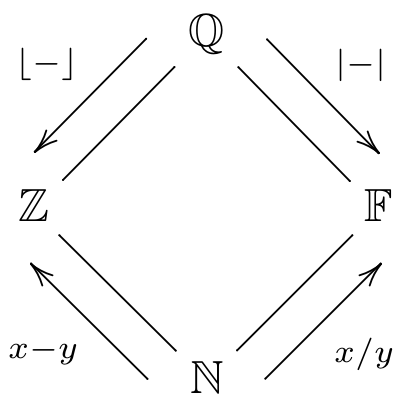
\includegraphics[width=0.3\textwidth]{../../docs/images/diamond.png}
  \caption{\disco's numeric type lattice}
  \label{fig:lattice}
\end{figure}
$\N$ is a subtype of both $\Z$ and $\F$, which are in turn both
subtypes of $\Q$.  Moving up and left in the lattice (from $\N$ to
$\Z$, or $\F$ to $\Q$) corresponds to allowing subtraction; moving up
and right corresponds to allowing division.  Moving down and left can
be accomplished via a rounding operation such as floor or ceiling;
moving down and right can be accomplished via absolute
value. \pref{lst:subtype} demonstrates these ideas by requesting the
types of various expressions.  In the last example, in particular,
notice how \disco infers the type $\Q$ for the elements of the list,
since that is the only type that supports both negation and division.
\begin{listing}
\begin{minted}{text}
Disco> :type -3
-3 : ℤ
Disco> :type |-3|
abs(-3) : ℕ
Disco> :type 2/3
2 / 3 : 𝔽
Disco> :type -2/3
-2 / 3 : ℚ
Disco> :type floor(-2/3)
floor(-2 / 3) : ℤ
Disco> :type [1,2,3]
[1, 2, 3] : List(ℕ)
Disco> :type [1,-2,3/5]
[1, -2, 3 / 5] : List(ℚ)
\end{minted}
\caption{Numeric types and subtyping}
\label{lst:subtype}
\end{listing}

\disco has no floating-point type, because floating-point numbers are
the worst \cite{goldberg1991every} and there is no particular need for real numbers
in a Discrete Mathematics course.


% \disco also has some operations which are less typical but
% particularly useful in a Discrete Mathematics context, such as
% factorial, binomial and multinomial coefficients, divisibility and
% primality testing, and factoring.

% \begin{verbatim}
% Disco> 50!
% 30414093201713378043612608166064768844377641568960512000000000000
% Disco> 10 choose 3
% 120
% Disco> 10 choose [3,5,2]
% 2520
% Disco> 13 divides 91
% true
% Disco> import num
% Loading num.disco...
% Disco> factor(2520)
% ⟅2 # 3, 3 # 2, 5, 7⟆
% \end{verbatim}

\section{Syntax}

For the most part, \disco tries to use syntax as close to standard
mathematical syntax as possible.  However, there are a few notable
cases where this was deemed impossible, typically because standard
mathematical syntax is particularly ambiguous or overloaded.  Thinking
about these cases is worthwhile, since they are likely to confuse
students anyway.

\begin{itemize}
\item Mathematicians are very fond of using vertical bars for multiple
  unrelated things, and \disco actually does well to allow them in
  many cases: absolute value, set cardinality, and the separator
  between expression and guards in a comprehension all can be written
  in \disco with vertical bars.  However, the ``evenly divides''
  relation is also traditionally written with a vertical bar, as in $3
  \mid 21$, but \disco does not support this notation.  Including it
  makes the grammar extremely ambiguous.  (And besides, Dijkstra tells
  us that we should not use a physically symmetric operator symbol for
  a nonsymmetric relation! \todo{cite}) Instead, \disco provides
  \texttt{divides} as an infix operator.  In my experience students
  had no problem remembering the difference.
\item The equality symbol $=$ is also overloaded to denote both
  definition and equality testing.  Disco cannot use the same symbol
  for both, since otherwise it would be impossible to tell whether the
  user is writing a definition or entering a Boolean test to be
  evaluated.
\item \disco allows juxtaposition to denote both function application,
  as in \texttt{f(3)}, and multiplication, as in \texttt{2x}.  It uses
  a simple syntax-directed approach to tell them apart: if the
  expression on the left-hand side of a juxtaposition is a numeric
  literal, or a parenthesized expression with an operator, then it is
  interpreted as multiplication; otherwise it is interpreted as
  function application.  However, this does not always get it right,
  and there are times when an explicit multiplication operator must be
  written.  It might be worth exploring a more type-directed approach,
  although that would be considerably more complex.  It seems like to
  really get this ``right'' requires general intelligence: for
  example, does the expression $f(x+2)$ denote multiplication or
  function application?  Are you sure?  How do you know?  What about
  in the expression $x(y+2)$?  Or how about ``Let $x$ be the function
  which doubles its argument, and consider $x(y+2)$ \dots''?
\end{itemize}

\section{Types}
\label{sec:types}

\section{Tooling}
\label{sec:tools}

\section{Discussion}
\label{sec:discussion}


\section{Acknowledgements}
\label{sec:acks}

Harley Eades, Callahan Hirrel, Bosco Ndemeye, Sanjit Kalapatapu, Jacob
Hines, Daniel Burnett

% The optional arguments of {\ttfamily $\backslash$documentclass$\{$eptcs$\}$} are
% \begin{itemize}
% \item at most one of
% {\ttfamily adraft},
% {\ttfamily submission} or
% {\ttfamily preliminary},
% \item at most one of {\ttfamily publicdomain} or {\ttfamily copyright},
% \item and optionally {\ttfamily creativecommons},
%   \begin{itemize}
%   \item possibly augmented with
%     \begin{itemize}
%     \item {\ttfamily noderivs}
%     \item or {\ttfamily sharealike},
%     \end{itemize}
%   \item and possibly augmented with {\ttfamily noncommercial}.
%   \end{itemize}
% \end{itemize}
% We use {\ttfamily adraft} rather than {\ttfamily draft} so as not to confuse hyperref.
% The style-file option {\ttfamily submission} is for papers that are
% submitted to {\ttfamily $\backslash$event}, where the value of the latter is
% to be filled in in line 2 of the tex file. Use {\ttfamily preliminary} only
% for papers that are accepted but not yet published. The final version
% of your paper to be uploaded to the EPTCS website should have
% none of these style-file options.

% Using the style-file option
% \href{http://creativecommons.org/licenses/}{creativecommons}
% authors equip their paper with a Creative Commons license that allows
% everyone to copy, distribute, display, and perform their copyrighted
% work and derivative works based upon it, but only if they give credit
% the way you request. By invoking the additional style-file option {\ttfamily
% noderivs} you let others copy, distribute, display, and perform only
% verbatim copies of your work, but not derivative works based upon
% it. Alternatively, the {\ttfamily sharealike} option allows others to
% distribute derivative works only under a license identical to the
% license that governs your work. Finally, you can invoke the option
% {\ttfamily noncommercial} that let others copy, distribute, display, and
% perform your work and derivative works based upon it for
% noncommercial purposes only.

% Authors' (multiple) affiliations and emails use the commands
% {\ttfamily $\backslash$institute} and {\ttfamily $\backslash$email}.
% Both are optional.
% Authors should moreover supply
% {\ttfamily $\backslash$titlerunning} and {\ttfamily $\backslash$authorrunning},
% and in case the copyrightholders are not the authors also
% {\ttfamily $\backslash$copyrightholders}.
% As illustrated above, heuristic solutions may be called for to share
% affiliations. Authors may apply their own creativity here \cite{multipleauthors}.

% EPTCS recommends using {\ttfamily $\backslash$documentclass[copyright,creativecommons]\{eptcs\}}.\\
% Additionally, the title should be set in \href{https://en.wikipedia.org/wiki/Title_case}{title case},
% meaning that major words start with a capital letter, and only articles, prepositions and
% conjunctions appear in lower case.

% \section{Ancillary files}

% Authors may upload ancillary files to be linked alongside their paper.
% These can, for instance, contain raw data for tables and plots in the
% article or program code.  Ancillary files are included with an EPTCS
% submission by placing them in a directory \texttt{anc} next to the
% main latex file. See also \url{https://arxiv.org/help/ancillary_files}.
% Please add a file README in the directory \texttt{anc}, explaining the
% nature of the ancillary files, as in
% \url{http://eptcs.org/paper.cgi?226.21}.

% \section{Prefaces}

% Volume editors may create prefaces using this very template,
% with {\ttfamily $\backslash$title$\{$Preface$\}$} and {\ttfamily $\backslash$author$\{\}$}.

\section{Bibliography}

% We request that you use
% \href{http://eptcs.web.cse.unsw.edu.au/eptcs.bst}
% {\ttfamily $\backslash$bibliographystyle$\{$eptcs$\}$}
% \cite{bibliographystylewebpage}, or one of its variants
% \href{http://eptcs.web.cse.unsw.edu.au/eptcsalpha.bst}{eptcsalpha},
% \href{http://eptcs.web.cse.unsw.edu.au/eptcsini.bst}{eptcsini} or
% \href{http://eptcs.web.cse.unsw.edu.au/eptcsalphaini.bst}{eptcsalphaini}
% \cite{bibliographystylewebpage}. Compared to the original {\LaTeX}
% {\ttfamily $\backslash$biblio\-graphystyle$\{$plain$\}$},
% it ignores the field {\ttfamily month}, and uses the extra
% bibtex fields {\ttfamily eid}, {\ttfamily doi}, {\ttfamily eprint} and {\ttfamily url}.
% The first is for electronic identifiers (typically the number $n$
% indicating the $n^\mathrm{th}$ paper in an issue) of papers in electronic
% journals that do not use page numbers. The other three are to refer,
% with life links, to electronic incarnations of the paper.

% \paragraph{DOIs}

% Almost all publishers use digital object identifiers (DOIs) as a
% persistent way to locate electronic publications. Prefixing the DOI of
% any paper with {\ttfamily https://doi.org/} yields a URI that resolves to the
% current location (URL) of the response page\footnote{Nowadays, papers
%   that are published electronically tend
%   to have a \emph{response page} that lists the title, authors and
%   abstract of the paper, and links to the actual manifestations of
%   the paper (e.g., as {\ttfamily dvi} or {\ttfamily pdf} file). Sometimes
%   publishers charge money to access the paper itself, but the response
%   page is always freely available.}
% of that paper. When the location of the response page changes (for
% instance, through a merge of publishers), the DOI of the paper remains
% the same and (through an update by the publisher) the corresponding
% URI will then resolve to the new location. For that reason, a reference
% ought to contain the DOI of a paper, with a live link to the corresponding
% URI, rather than a direct reference or link to the current URL of the
% publisher's response page. This is the r\^ole of the bibtex field {\ttfamily doi}.
% {\bfseries EPTCS requires the inclusion of a DOI in each cited paper, when available.}

% DOIs of papers can often be found through
% \url{http://www.crossref.org/guestquery};\footnote{For papers that will appear
%   in EPTCS and use \href{http://eptcs.web.cse.unsw.edu.au/eptcs.bst}
%   {\ttfamily $\backslash$bibliographystyle$\{$eptcs$\}$} there is no need to
%   find DOIs on this website, as EPTCS will look them up for you
%   automatically upon submission of the first version of your paper;
%   these DOIs can then be incorporated into the final version, together
%   with the remaining DOIs that need to be found at DBLP or the publisher's web pages.}
% the second method {\itshape Search on article title}, only using the {\bfseries
% surname} of the first-listed author, works best.
% Other places to find DOIs are DBLP and the response pages for cited
% papers (maintained by their publishers).

% \paragraph{The bibtex fields {\ttfamily eprint} and {\ttfamily url}}

% Often an official publication is only available against payment. However,
% as a courtesy to readers that do not wish to pay, the authors also
% make the paper available free of charge at a repository such as
% \url{arXiv.org}. In such a case, it is recommended to also refer and
% link to the URL of the response page of the paper in such a
% repository.  This can be done using the bibtex fields {\ttfamily eprint}
% or {\ttfamily url}.  The latter field should \textbf{not} be used
% to duplicate information that is also provided through {\ttfamily doi} or {\ttfamily eprint}.
% You can find archival-quality URLs for most recently published papers
% in DBLP, but please suppress repetition of DOI or {\ttfamily eprint} information though {\ttfamily url}.
% In fact, it is often useful to check your references against DBLP records anyway,
% or just find them there in the first place.

% \paragraph{Typesetting DOIs and URLs}

% When using {\LaTeX} rather than {\ttfamily pdflatex} to typeset your paper, by
% default no line breaks within long URLs are allowed. This leads often
% to very ugly output, that moreover is different from the output
% generated when using {\ttfamily pdflatex}. This problem is repaired when
% invoking \href{http://eptcs.web.cse.unsw.edu.au/breakurl.sty}
% {\ttfamily $\backslash$usepackage$\{$breakurl$\}$}: it allows line breaks
% within links and yield the same output as obtained by default with
% {\ttfamily pdflatex}.
% When invoking {\ttfamily pdflatex}, the package {\ttfamily breakurl} is ignored.

% The package {\ttfamily $\backslash$usepackage$\{$underscore$\}$} is
% recommended to deal with underscores in DOIs. This is not needed when
% using {\ttfamily $\backslash$usepackage$\{$breakurl$\}$} and not {\ttfamily pdflatex}.

% \paragraph{References to papers in the same EPTCS volume}

% To refer to another paper in the same volume as your own contribution,
% use a bibtex entry with
% \begin{center}
%   {\ttfamily series    = $\{\backslash$thisvolume$\{5\}\}$},
% \end{center}
% where 5 is the submission number of the paper you want to cite.
% You may need to contact the author, volume editors, or EPTCS staff to
% find that submission number; it becomes known (and unchangeable)
% as soon as the cited paper is first uploaded at EPTCS\@.
% Furthermore, omit the fields {\ttfamily publisher} and {\ttfamily volume}.
% Then in your main paper, you put something like:

% \noindent
% {\small \ttfamily $\backslash$providecommand$\{\backslash$thisvolume$\}$[1]$\{$this
%   volume of EPTCS, Open Publishing Association$\}$}

% \noindent
% This acts as a placeholder macro-expansion until EPTCS software adds
% something like

% \noindent
% {\small \ttfamily $\backslash$newcommand$\{\backslash$thisvolume$\}$[1]%
%   $\{\{\backslash$eptcs$\}$ 157$\backslash$opa, pp 45--56, doi:\dots$\}$},

% \noindent
% where the relevant numbers are pulled out of the database at publication time.
% Here the newcommand wins from the providecommand, and {\ttfamily \small $\backslash$eptcs}
% resp.\ {\ttfamily \small $\backslash$opa} expand to

% \noindent
% {\small \ttfamily $\backslash$sl Electronic Proceedings in Theoretical Computer Science} \hfill and\\
% {\small \ttfamily , Open Publishing Association} \hfill .

% \noindent
% Hence putting {\small \ttfamily $\backslash$def$\backslash$opa$\{\}$} in
% your paper suppresses the addition of a publisher upon expansion of the citation by EPTCS\@.
% An optional argument like
% \begin{center}
%   {\ttfamily series    = $\{\backslash$thisvolume[EPTCS]$\{5\}\}$},
% \end{center}
% overwrites the value of {\ttfamily \small $\backslash$eptcs}.

% \nocite{*}
\bibliographystyle{eptcsalpha}
\bibliography{references}
\end{document}
